\chapter{The Large Hadron Collider and the \ATLAS Detector}\label{chap:lhc_atlas}

The Large Hadron Collider (\LHC) at \CERN has extended the frontiers of particle physics through its unprecedented energy and luminosity.
In 2010, the \LHC collided proton bunches, each containing more than $10^{11}$ particles, 20 million times per second, providing \SI{7}{\TeV} proton-proton collisions at instantaneous luminosities of up to \peakLumi.
In 2015, Run 2 happened.
2022 marked the beginning of Run 3 with higher peak lumis\dots


\section{The ATLAS Detector}\label{sec:atlas_detector}
%% from https://twiki.cern.ch/twiki/bin/view/AtlasProtected/PubComCommonText

% Footnote with ATLAS coordinate system
\newcommand{\AtlasCoordFootnote}{%
ATLAS uses a right-handed coordinate system with its origin at the nominal interaction point in the centre of the detector and the \(z\)-axis along the beam pipe. The \(x\)-axis points from the interaction point to the centre of the LHC ring, and the \(y\)-axis points upwards. Cylindrical coordinates \((r,\phi)\) are used in the transverse plane, \(\phi\) being the azimuthal angle around the \(z\)-axis. The pseudorapidity is defined in terms of the polar angle \(\theta\) as \(\eta = -\ln \tan(\theta/2)\). Angular distance is measured in units of \(\DeltaR \equiv \sqrt{(\Delta\eta)^{2} + (\Delta\phi)^{2}}\).}

The ATLAS detector at the LHC covers nearly the entire solid angle around the collision point.\footnote{\AtlasCoordFootnote}
It consists of an inner tracking detector surrounded by a thin superconducting solenoid, electromagnetic and hadron calorimeters,
and a muon spectrometer incorporating three large superconducting air-core toroidal magnets.

The inner-detector system (ID) is immersed in a \SI{2}{\tesla} axial magnetic field 
and provides charged-particle tracking in the range \(|\eta| < 2.5\).
The high-granularity silicon pixel detector covers the vertex region and typically provides four measurements per track, 
the first hit normally being in the insertable B-layer (IBL) installed before Run~2~\cite{ATLAS-TDR-19,PIX-2018-001}.
It is followed by the silicon microstrip tracker (SCT), which usually provides eight measurements per track.
These silicon detectors are complemented by the transition radiation tracker (TRT),
which enables radially extended track reconstruction up to \(|\eta| = 2.0\). 
The TRT also provides electron identification information 
based on the fraction of hits (typically 30 in total) above a higher energy-deposit threshold corresponding to transition radiation.
Reconstructed charged particles are assumed to have a charge of $\pm 1$.

The calorimeter system covers the pseudorapidity range \(|\eta| < 4.9\).
Within the region \(|\eta|< 3.2\), electromagnetic calorimetry is provided by barrel and 
endcap high-granularity lead/liquid-argon (LAr) calorimeters,
with an additional thin LAr presampler covering \(|\eta| < 1.8\)
to correct for energy loss in material upstream of the calorimeters.
Hadron calorimetry is provided by the steel/scintillator-tile calorimeter,
segmented into three barrel structures within \(|\eta| < 1.7\), and two copper/LAr hadron endcap calorimeters.
The solid angle coverage is completed with forward copper/LAr and tungsten/LAr calorimeter modules
optimised for electromagnetic and hadronic energy measurements respectively.

The muon spectrometer (MS) comprises separate trigger and
high-precision tracking chambers measuring the deflection of muons in a magnetic field generated by the superconducting air-core toroidal magnets.
The field integral of the toroids ranges between \num{2.0} and \SI{6.0}{\tesla\metre}
across most of the detector. 
Three layers of precision chambers, each consisting of layers of monitored drift tubes, covers the region \(|\eta| < 2.7\),
complemented by cathode-strip chambers in the forward region, where the background is highest.
The muon trigger system covers the range \(|\eta| < 2.4\) with resistive-plate chambers in the barrel, and thin-gap chambers in the endcap regions.

Interesting events are selected by the first-level trigger system implemented in custom hardware,
followed by selections made by algorithms implemented in software in the high-level trigger~\cite{TRIG-2016-01}. 
The first-level trigger accepts events from the \SI{40}{\MHz} bunch crossings at a rate below \SI{100}{\kHz},
which the high-level trigger further reduces in order to record events to disk at about \SI{1}{\kHz}.

An extensive software suite~\cite{ATL-SOFT-PUB-2021-001} is used in the reconstruction and analysis of real
and simulated data, in detector operations, and in the trigger and data acquisition systems of the experiment.

A complete overview of the ATLAS detector is provided in Ref.~\cite{PERF-2007-01}.






High level information taken from \cite{PERF-2007-01}. Initial (circa 2000) information about each sub-detector system is available in the respective technical design reports (TDRs). Note that much of the specifics will therefore be outdated.

The detector is made up of several specialised subdetectors. In order of increasing radial distance from the point of particle interaction, these are:





\subsection{The Inner Detector}

% overfull hbox!
\begin{figure}[!htpb]
  \centering
  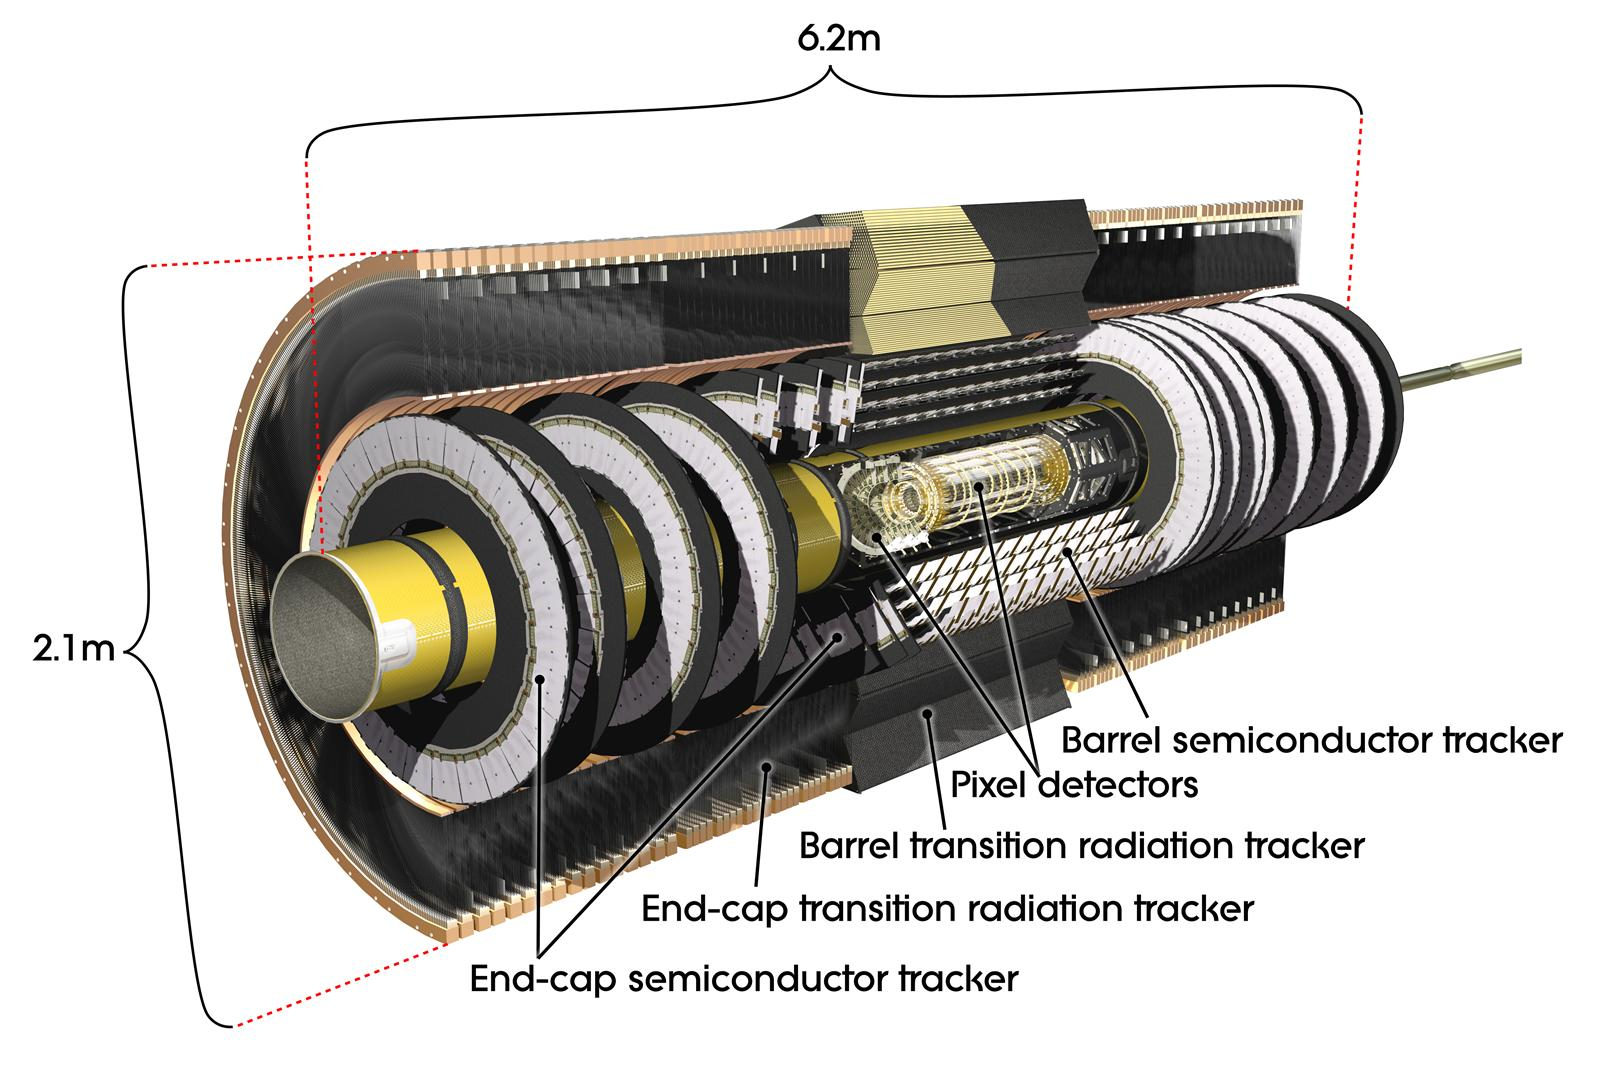
\includegraphics[width=0.4\linewidth]{chapters/2.detector/figs/atlas_id.jpg}
  \caption{The \ATLAS ID. After run 3, the ID will be replaced by the ITk.}
  \label{fig:atlas_id_run1}
\end{figure}



%
\begin{figure}[!htpb]
  \centering
  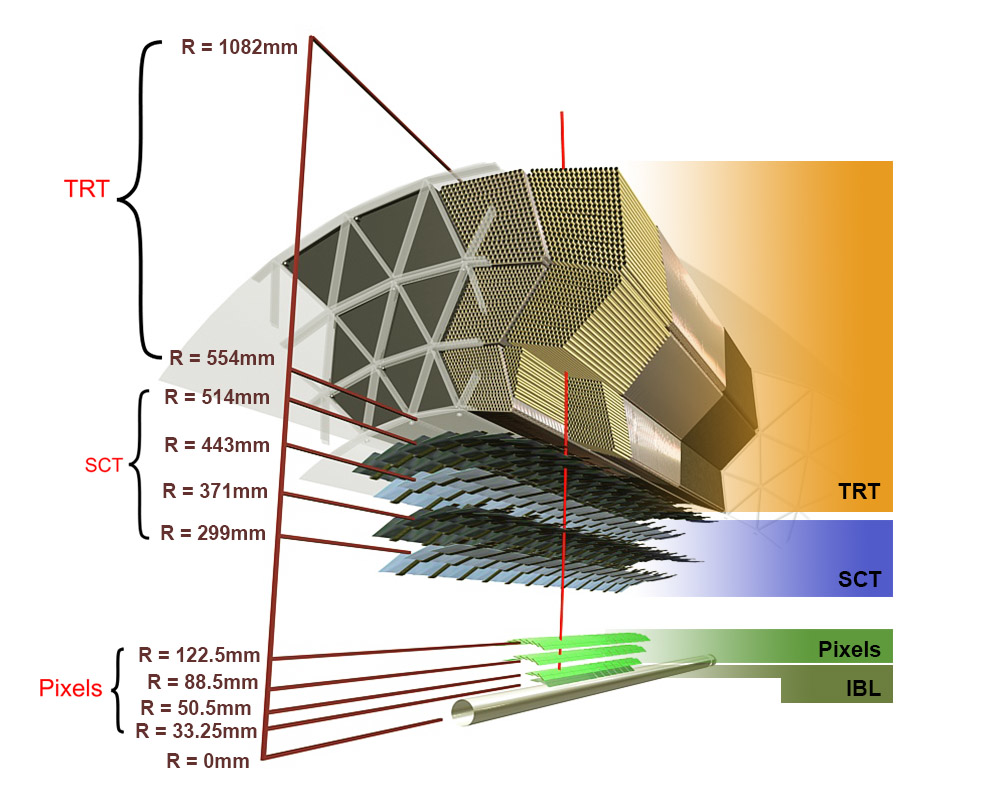
\includegraphics[width=0.4\linewidth]{chapters/2.detector/figs/atlas_id_xs.png}
  \caption{The \ATLAS ID. After run 3, the ID will be replaced by the ITk.}
  \label{fig:atlas_id_run2}
\end{figure}
%

High resolution tracking (coverage over $|\eta| < 2.5$) hardware, contained in a superconducting solenoidal magnet with a central field of 2T. Combination of the two systems below yields robust pattern recognition and high precision in both $\phi$ and $z$ coordinates.

Tracking is useful for: impact parameter measurements, vertexing for heavy-flavour and $\tau$ tagging. Momentum resolution is sufficient to identify the charge sign of particles up to the highest energies expected at LHC. After run 3, the ID will be replaced by the ITk.


\subsubsection{Pixel Layers}
Arranged in three cylindrical barrels at increasing radio ( 4, 11, 14 cm), and four discs on each side. Radiation hardened readout electronics. Full angular coverage. 140 million readout channels. The specification determines the impact parameter resolution and the ability of the ID to find short-lived particles such as b-quarks and $\tau$-leptons. Silicon pixels.The pixel detector dominates measurements of track impact parameters and provides vertex reconstruction capabilities. Table 2.2 summarises the main features of the pixel subsystem. Each pixel module is required to have a high granularity (resolution) to maintain a low occupancy (high sparsity to resolve different tracks). The pixel layers consist of the three original barrels and three disks (end-caps), and a new IBL. In order of increasing radius from the beam-line the pixel detector consists of the following layers

Insertable B-Layer (IBL). The innermost layer of pixel detectors, 3.3cm from beam axis. Added in 2014. It was built to cope with high radiation and occupancy, and is the first large scale application of 3D sensors and CMOS 130nm technology.

Three barrel layers: Layer 0 (also sometime called the b-layer or B-layer), Layer 1 and Layer 2. Additionally there two identical endcap regions, each with three disk layers.


\subsubsection{Semi-Conductor Tracker (SCT)}
Silicon microstrip detectors. Contributes to the measurement of momentum, impact parameter and vertex position. $61 ~\textrm{m}^2$ of silicon detector, 6.2 million readout channels.

\subsubsection{Transition Radiation Tracker (TRT)}
Continuous tracking using straw detectors. The straws run parallel to the $z$ axis and therefore the TRT only provides $R$\nobreakdash-$\phi$ information. Radial straws on the endcaps. Electron identification capability is added by employing xenon gas to detect transition-radiation photons created in a radiator between the straws. A good pattern recognition performance is assured by the continuous tracking. Within the radial space available, the straw spacing has been optimised for tracking at the expense of electron
identification, which would be improved by a greater path length through the radiator material and fewer active straws. The TRT contributes to the accuracy of the momentum measurement in the ID. It aids the pattern recognition by the addition of around 36 hits per track, and allows a simple and fast L2 track trigger to be implemented. It allows the ID to reconstruct $V_0$s which are especially interesting in CP-violating $B$ decays. In addition it provides additional discrimination between electrons and hadrons.


%
\begin{figure}[!htpb]
  \centering
  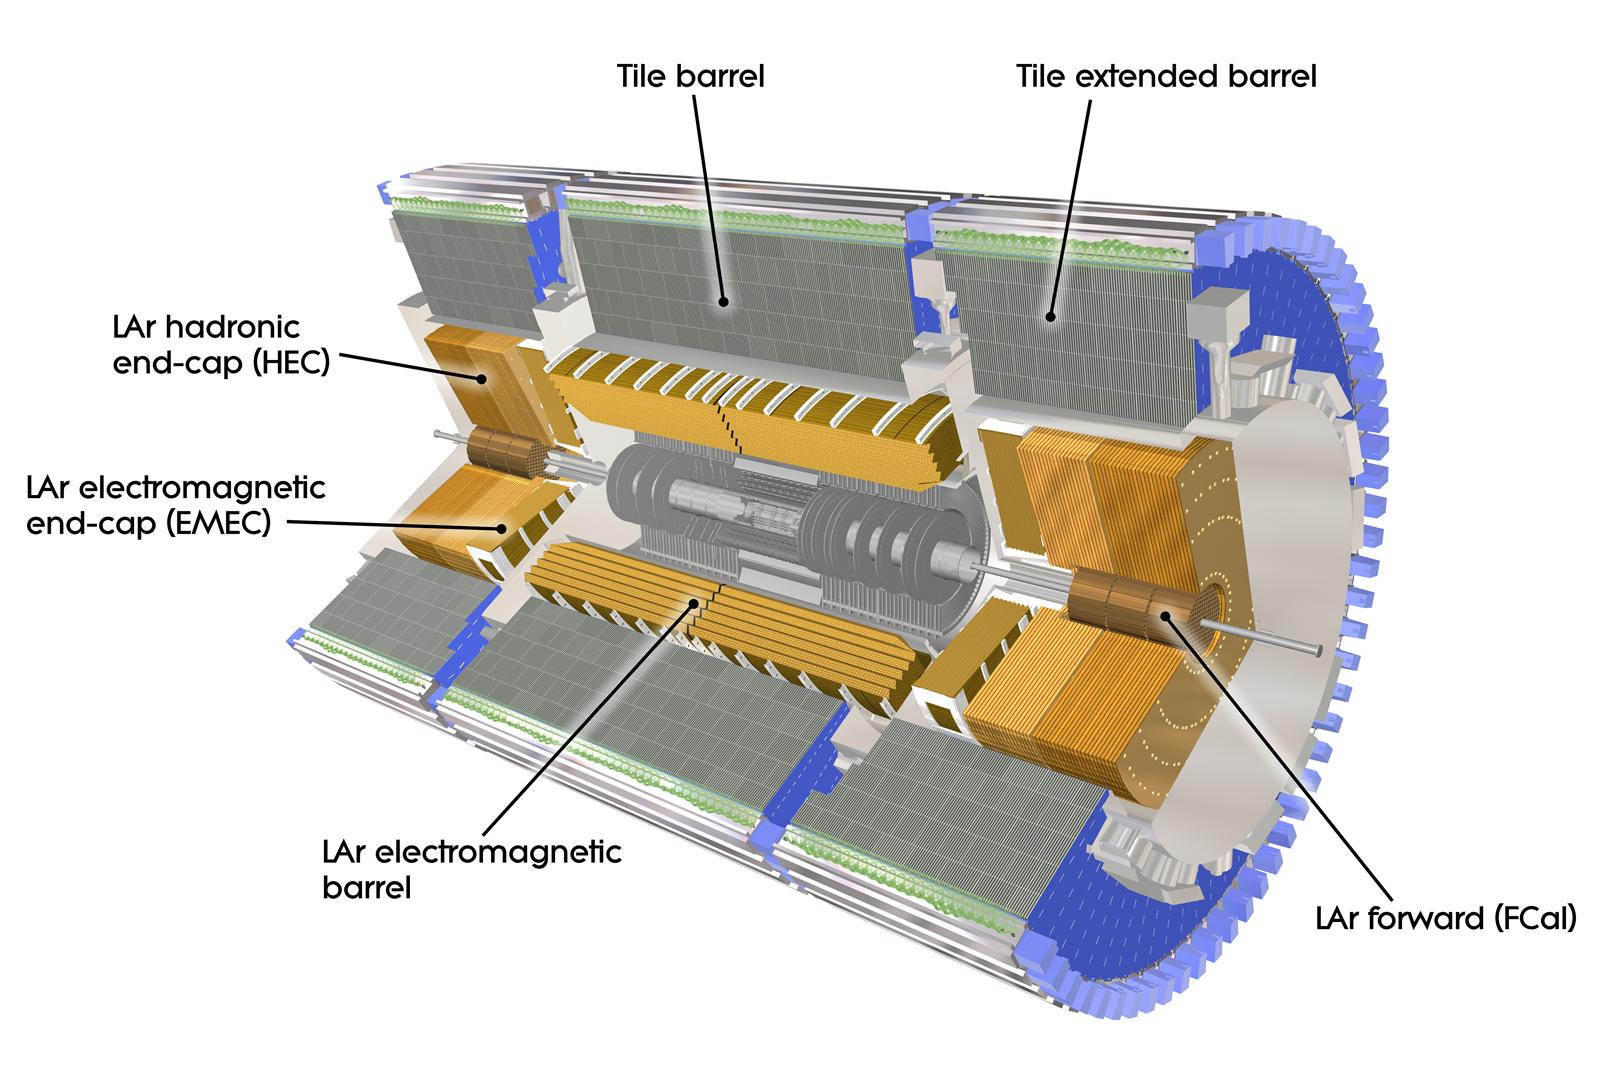
\includegraphics[width=0.4\linewidth]{chapters/2.detector/figs/atlas_calos.jpg}
  \caption{The \ATLAS calorimeters. The ECal (orange) and HCal (grey, dark orange).}
  \label{fig:atlas_calos}
\end{figure}
%



\subsection{Calorimeters}

Calorimeters measure the energy of particle passing through them. They cover $|\eta| < 4.9$ using a range of different techniques depending on the location in $\eta$. Over the $\eta$ region matched to the inner detector, the fine granularity of the EM calorimeter is ideally suited for precision measurements of electrons and photons. The coarser granularity of the rest of the calorimeter is sufficient to satisfy the physics requirements for jet reconstruction and $E_T^{\textrm{miss}}$ measurements. Particles entering the calorimeter, will cause a particle shower inside the calorimeter. Calorimeters must provide good containment for electromagnetic and hadronic showers, and must also limit punch-through (leakage of non muon particles) into the muon system (dependent on the radial depth of the calorimeter system). The calorimeters measure the energies and positions of electrons, photons and jets. In doing so they stop these particles penetrating into the muon spectrometer. When a relativistic photon or electron is incident on a thick absorber, it initiates an electromagnetic cascade, generating secondary photons by bremsstrahlung ($e \rightarrow e\gamma$) and electrons by pair production ($\gamma \rightarrow e^+ e^- $).
    
A narrow transverse profile is characteristic of an electromagnetic cascade. Hadrons passing through matter also initiate cascades through inelastic hadron-nuclei interactions. The shower produces secondary hadrons and leptons and has a comparatively wide transverse profile. The nuclear interaction length is about an order of magnitude greater than the radiation length of the material. Therefore, like most general purpose experiments, ATLAS uses two different calorimetry systems to measure electrons and photons (the ECal) and hadrons (the HCal). 

\subsubsection{Liquid Argon (LAr) Electromagnetic (EM) Calorimeter (Ecal)}
The EM calorimeter is divided into a barrel part ($|\eta| < 1.475$) and two end-cap components ($1.375 < |\eta| < 3.2$), each housed in their own cryostat. The EM calorimeter is a lead-LAr detector with accordion-shaped kapton electrodes and lead absorber plates over its full coverage. The accordion geometry provides complete $\phi$ symmetry without azimuthal cracks. Showers initiated in the lead produce secondary particles which ionise the liquid argon. The charge is collected on copper electrodes and read out. Additionally, multiple samplings of the shower are used to resolve its pointing vector.

\subsubsection{Hadronic calorimeters (HCal)}
The tile calorimeter is placed directly outside the EM calorimeter envelope. Its barrel covers the region $|\eta| < 1.0$, and its two extended barrels (larger $z$ displacement) the range $0.8 < |\eta| < 1.7$. It is a sampling calorimeter using steel as the absorber and scintillating tiles as the active material. The HCal barrel uses iron absorbers to initiate hadronic cascades and plastic scintillator tiles as the active

LAr hadronic end-cap calorimeter (HEC). Located directly behind (in $z$) the end-cap electromagnetic calorimeter and sharing the same LAr cryostats. The high level of radiation in the forward regions would cause severe damage to plastic scintillators. In the end-caps, parallel copper plates are submerged in liquid argon, which is preferred as the active medium because of its inherent radiation hardness.

LAr forward calorimeter (FCal).


\subsection{Muon System}

%
\begin{figure}[!htpb]
  \centering
  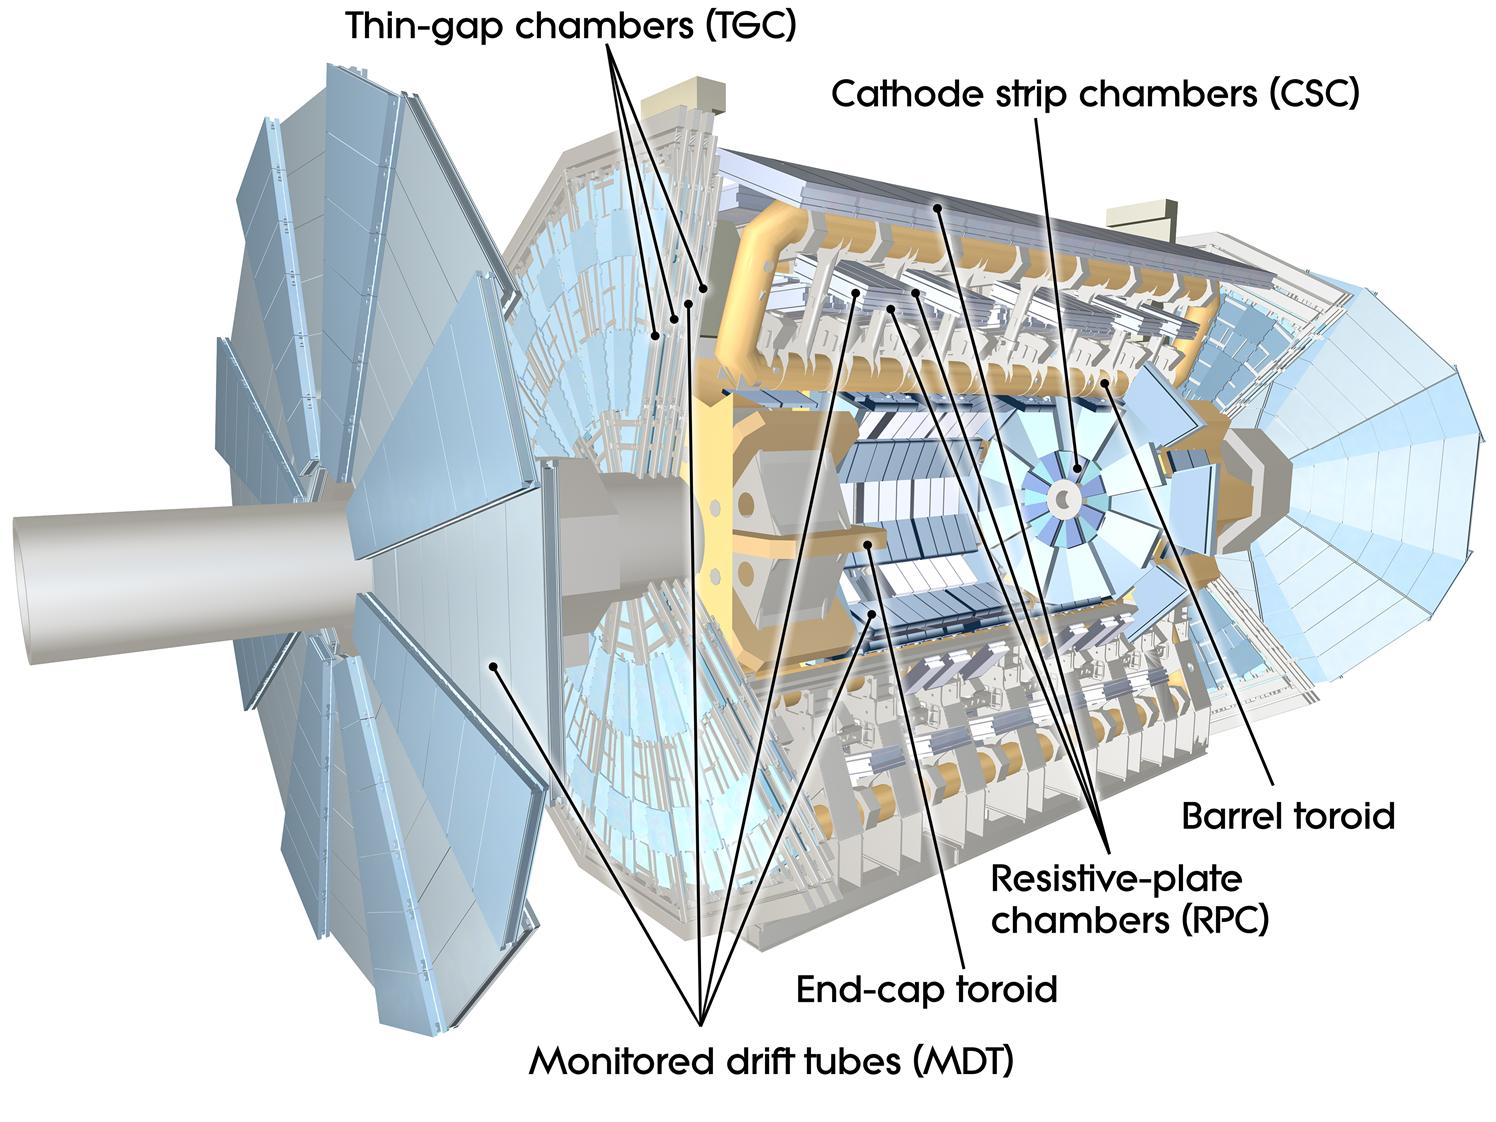
\includegraphics[width=0.4\linewidth]{chapters/2.detector/figs/atlas_muon_system.jpg}
  \caption{The \ATLAS muon detectors.}
  \label{fig:atlas_muon_system}
\end{figure}
%


Based on the magnetic deflection of muon tracks in the large superconducting air-core toroid magnets, instrumented with separate trigger and high-precision tracking chambers. This magnet configuration provides a field which is mostly orthogonal to the muon trajectories, while minimising the degradation of resolution due to multiple scattering. In the barrel region, tracks are measured in chambers arranged in three cylindrical layers around the beam axis; in the transition and end-cap regions, the chambers are installed in planes perpendicular to the beam, also in three layers.



\subsection{The Trigger}
\label{sec:bg-theory:triggers}
An LHCb trigger table borrowed from \texttt{hepthesis} is shown in \TableRef{tab:bg-theory:trigger_details}:

\begin{table}[bht]
  \footnotesize\centering
  \setlength{\tabcolsep}{0.5em} % for the horizontal padding
  \caption{Characteristics of the trigger levels and offline analysis.}
  \begin{tabular}{lllll}
                & L0              & L1              & HLT             \\
    \midrule
    Input rate  & \SI{40}{\MHz} & \SI{1}{\MHz}  & \SI{40}{\kHz} \\
    Output rate & \SI{1}{\MHz}  & \SI{40}{\kHz} & \SI{2}{\kHz}  \\
    Location    & On detector     & Counting room   & Counting room   \\
  \end{tabular}
  \label{tab:bg-theory:trigger_details}
\end{table}


\subsubsection{Triggers and Data Acquisition (TDAQ)}

The trigger system has three distinct levels: L1, L2, and the event filter. Each trigger level refines the decisions made at the previous level and, where necessary, applies additional selection criteria. The data acquisition system receives and buffers the event data from the detector-specific readout electronics, at the L1 trigger accept rate. The first level uses a limited amount of the total detector information to make a decision in in a short time.


\subsubsection{The Trigger System}

The L1 trigger searches for high transverse-momentum muons, electrons, photons, jets, and $\tau$-leptons decaying into hadrons, as well as large missing and total transverse energy. Its selection is based on information from a subset of detectors. High transverse-momentum muons are identified using trigger chambers in the barrel and end-cap regions of the spectrometer. Calorimeter selections are based on reduced-granularity information from all the calorimeters. Results from the L1 muon and calorimeter triggers are processed by the central trigger processor, which implements combinations of different trigger selections. In each event, the L1 trigger also defines one or more Regions-of-Interest (RoI’s), i.e. the geographical coordinates in $\eta$ and $\phi$, of those regions within the detector where its selection process has identified interesting features. The RoI data include information on the type of feature identified and the criteria passed, e.g. a threshold. This information is subsequently used by the high-level trigger.

The L2 selection is seeded by the RoI information provided by the L1 trigger. L2 selections use, at full granularity and precision, all the available detector data within the RoI’s (approximately 2\% of the total event data). The L2 menus are designed to reduce the trigger rate to approximately 3.5 kHz, with an event processing time of about 40 ms, averaged over all events. The final stage of the event selection is carried out by the event filter, which reduces the event rate to roughly 200 Hz. Its selections are implemented using offline analysis procedures within an average event processing time of the order of four seconds.








\section{Reconstructed Physics Objects}\label{sec:physics-objects}

\subsection{Tracks}\label{sec:tracks}

The trajectories of charged particles are reconstructed as tracks from the energy depositions (hits) of the particles as they traverse the sensitive elements of the inner detector.
Track selection follows the loose selection described in Ref.~\cite{ATL-PHYS-PUB-2020-014} and outlined in~\cref{tab:track_selections}, which was found to improve the flavour tagging performance compared to previous tighter selections, whilst ensuring good resolution of tracks and a low fake rate~\cite{PERF-2015-08}.
The transverse IP $d_0$ and longitudinal IP $z_0$ are measured with respect to the hard scatter primary vertex, defined as the reconstructed primary vertex (PV) with the largest sum of the transverse momentum ($\pt$) of the associated tracks squared, $\sum \pt^2$.
%The reconstructed tracks are required to satisfy the quality requirements in \cref{tab:track_selections}.

\begin{table}[!htbp]
  \footnotesize\centering
  \setlength{\tabcolsep}{0.5em} % for the horizontal padding
  \caption{
    Quality selections applied to tracks,
    where $d_0$ is the transverse IP of the track, $z_0$ is the longitudinal IP with respect to the PV and $\theta$ is the track polar angle.
    Shared hits are hits used on multiple tracks which have not been classified as split by the cluster-splitting neural networks~\cite{PERF-2015-08}.
    Shared hits on pixel layers are given a weight of 1, while shared hits in the SCT are given a weight of 0.5.
    A hole is a missing hit, where one is expected, on a layer between two other hits on a track.
    }
  \begin{tabular}{ll}
    \toprule 
    \textbf{Parameter} & \textbf{Selection} \\
    \hline
    $\pt$                & $> 500$ MeV \\
    $|d_0|$              & $< 3.5$ mm \\
    $|z_0 \sin\theta|$   & $< 5$ mm \\
    Silicon hits         & $\ge 8$ \\
    Shared silicon hits  & $< 2$ \\
    Silicon holes        & $< 3$ \\
    Pixel holes          & $< 2$ \\
    \bottomrule
  \end{tabular}
  \vspace{4mm}
  \label{tab:track_selections}
\end{table}


\subsection{Jets}\label{sec:jets}

Jets are reconstructed from particle-flow objects \cite{PERF-2015-09} using the anti-$k_T$ algorithm \cite{Cacciari:2008gp} with a radius parameter of $0.4$.
The jet energy scale is calibrated according to Ref.~\cite{PERF-2016-04}.
Jets are also required not to overlap with a generator-level electron or muon from \Wboson boson decays.
All jets are required to have a pseudorapidity $|\eta| < 2.5$ and $\pt > \SI{20}{\GeV}$. 
Additionally, a standard selection using the Jet Vertex Tagger (JVT) algorithm at the tight working point is applied to jets with $\pt < \SI{60}{\GeV}$ and $|\eta| < 2.4$ in order to suppress pileup contamination \cite{ATLAS-CONF-2014-018}.
Tracks are associated to jets using a \DeltaR association cone, the width of which decreases as a function of jet \pt, with a maximum cone size of $\DeltaR \approx 0.45$ for jets with $\pt = \SI{20}{\GeV}$ and minimum cone size of $\DeltaR \approx 0.25$ for jets with $\pt > \SI{200}{\GeV}$. 
If a track is within the association cones of more than one jet, it is assigned to the jet which has a smaller $\DeltaR(\text{track}, \text{jet})$.

Jet flavour labels are assigned according to the presence of a truth hadron within ${\DeltaR(\text{hadron},\text{jet})<0.3}$ of the jet axis. If a \bhadron is found the jet is labelled a \bjet. In the absence of a \bhadron, if a \chadron is found the jet is called a \cjet.
If no \borchadrons are found, but a $\tau$ is found in the jet, it is labelled as a $\tau$-jet, else it is labelled as a \ljet.


\begin{itemize}
  \item Jet finding algorithms
\end{itemize}



\subsection{Leptons}\label{sec:leptons}